\section{Background}
Robots and human working in the same environment are increasing such as KAWADA Robotics NEXTAGE, a humanoid appearance manipulator design to perform tasks near human. Robots that are designed to work closely to human activity must consider, in addition to safety, how to convey information from human to robot. In general, this is usually done by sending command using an external controller; however this method does not always determine efficiency as it requires human to learn how to operate the robot beforehand. 

Intuitively, human have several means to communicate with each other such as visual and auditory communication. Physical communication is once such method. An example of physical communication would be a father guides their child by holding hands or a dog being pulled away on their leash by their owner. Communication through �eeffort�f or force is thought to be simpler method of communicating comparing to visual and auditory communication as learning feedback can directly occur without any prerequisite information unlike visual and auditory communication.

Using the same concept as above, this research attempts to mimic human's physical communication  on a robot by attempting to induce a wheeled robot with manipulator using human force as describe in figure \ref{fig:overview}.

\begin{figure}[!h]
\begin{center}
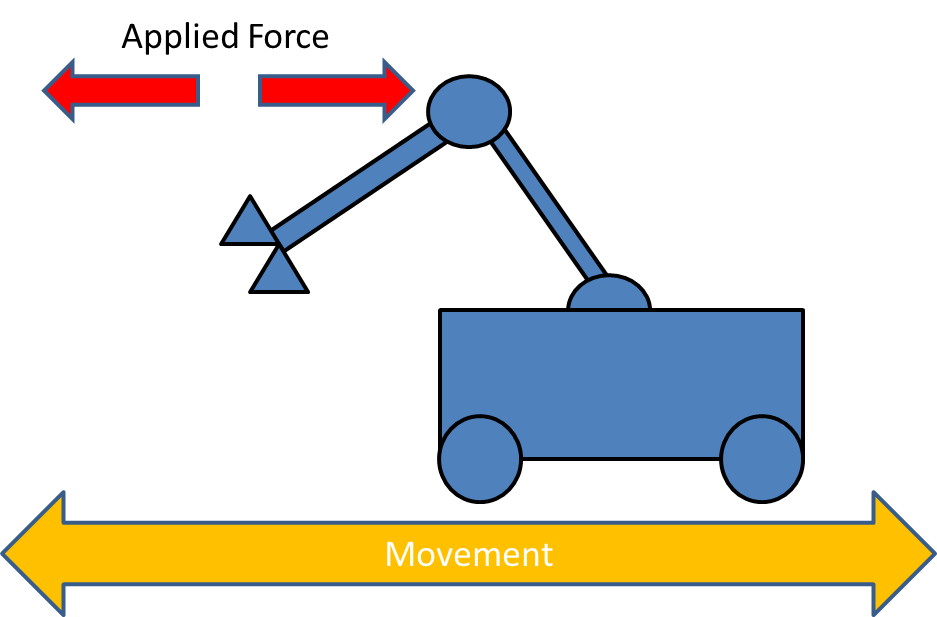
\includegraphics[width=7cm]{overview.png}
\caption{concept overview}
\label{fig:overview}
\end{center}
\end{figure}